\chapter{The Lifetime of Objects}

It would be great if programmers could be in charge only of hooking together and
populating their data structures, leaving the \jre responsible for the details
of object allocation and reclamation. The Java runtime does indeed help manage some
aspects of these management tasks, but leaves a good deal of work in your hands.
In Java, you needn't explicitly free objects, and in that way a managed language
is a big step up from a language like C. However, the ultimate promise of
automatic memory management, that you can create objects without regard for messy
details of storage management, doesn't play out ideally in practice. Unless you
are careful, your program will suffer from bugs such as memory leaks, and suffer
from poor performance. Sometimes, your objects don't easily fit into the limits
of a single Java process, and you need to manage, explicitly, shuttling them in
and out of the Java heap.

When programming in Java it is important to plan out the lifetime of your
objects. Your application needs some objects to live forever and it needs the
rest to die a timely death. This often requires careful design on your part, both
to avoid bugs and so that your application performs well in the case when not
everything fits into the Java heap. Designing a lifetime management strategy
usually requires that you take the tools that Java provides, and combine them
with other strategies implemented on top of Java.

\section{The Lifecycle of an Object}
%Every object created by your application lives for an interval of time from its
%creation to the point that the Java runtime gets around to collecting it. An object's {\em natural} lifetime is defined by the
%interval of time between its first and last necessary use. %cite drag paper
%here?

In a \emph{well-behaved} application, an object's lifetime spans its allocation,
use, and the short period, after its last use, during whch the \jre takes
control and eventually reclaims the space. For some subset of an object's {\em actual}
lifetime, that is the time from creation to reclamation, your application will
make use of the data stored in its fields.
\autoref{fig:typical-lifecycle} illustrates the lifecycle of a typical
object in a well behaved application.

\begin{figure}
	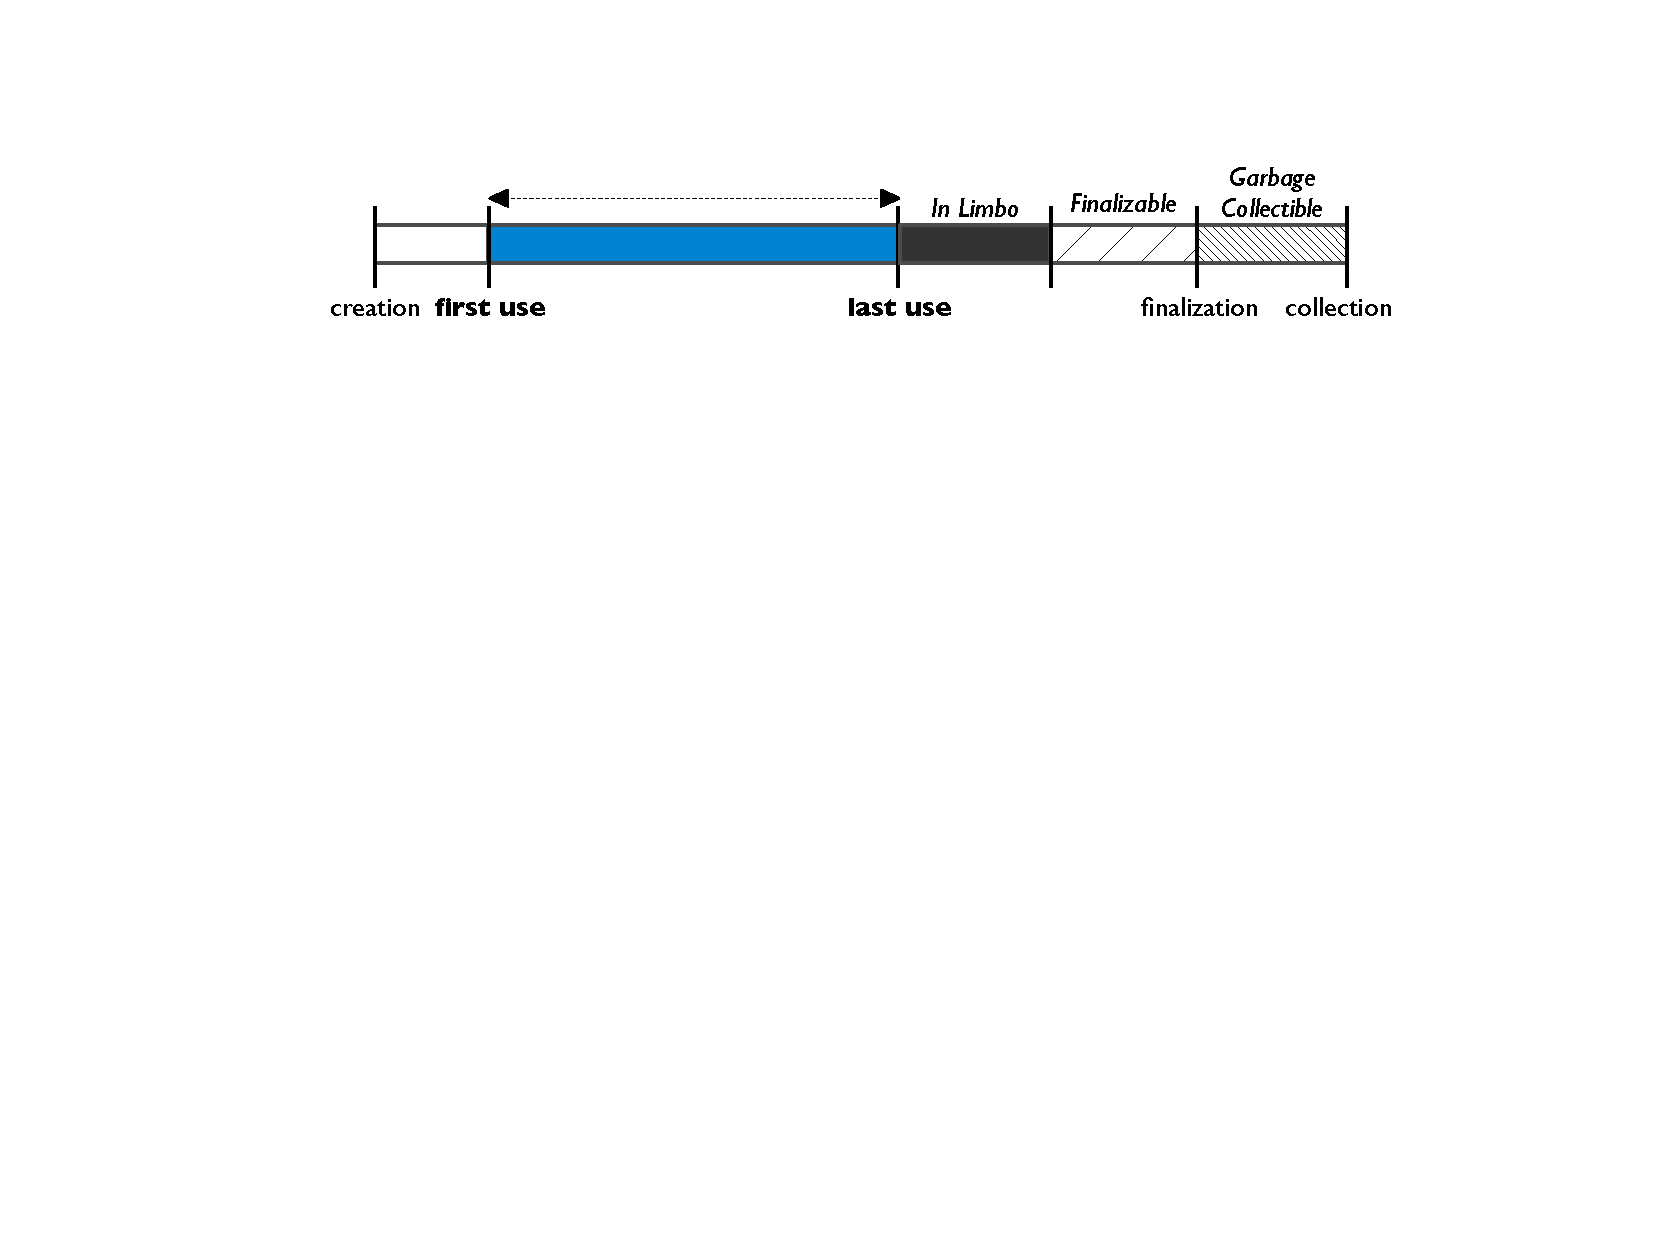
\includegraphics[width=0.9\textwidth]{Figures/lifetime/object-lifecycle}
	\caption{A timeline of the life of an object.}
	\label{fig:typical-lifecycle}
\end{figure}

\begin{example}{Parsing a Date} Consider a loop that 
shows a easy way to parse a list of dates.
\begin{shortlisting}
	for (String string : inputList) {
		ParsePosition pos = new ParsePosition(0);
		SimpleDateFormat parser = new SimpleDateFormat();
		System.out.println(parser.parse(string, pos));
	}
\end{shortlisting}
For each iteration of this loop, this code takes a date that is represented as a
string and produces a standard Java \class{Date} object. In doing so, a number of
objects are created. Two of these are easy to see, in the two \code{new} calls
that create the parse position and date parser objects. The programmer who wrote
this created two objects, but many more are created by the standard libraries to
finish the task. These include a calendar object, number of arrays, and the
\class{Date} itself. None of these objects are used beyond the iteration of the
loop in which they were created. Within one iteration, they are created, almost
immediately used, and then enter a state of \emph{limbo}.

\callout{limbo}{Objects in Limbo}{
In limbo, an object will never be used again, or at least not for long time,
but the \jre doesn't yet know that this is the case. The object hangs
around, taking up space in the Java heap until the point when it exits limbo.}

The \code{pos} object represents to the parser the position within the
input string to begin parsing. The implementation of the \code{parse} method
uses it early on in the process of parsing. Despite being unused for the
remainder of the parsing, the \jre does not know this until the current
iteration of the loop has finished. This time in limbo also includes the
entirety of the call to \code{System.out.println}, an operation entirely
unrelated to the creation or use of the parse position object. Once the current
loop iteration finishes, these two objects will exit limbo, and become garbage
collectible.
\end{example}

\begin{figure}
	\centering
	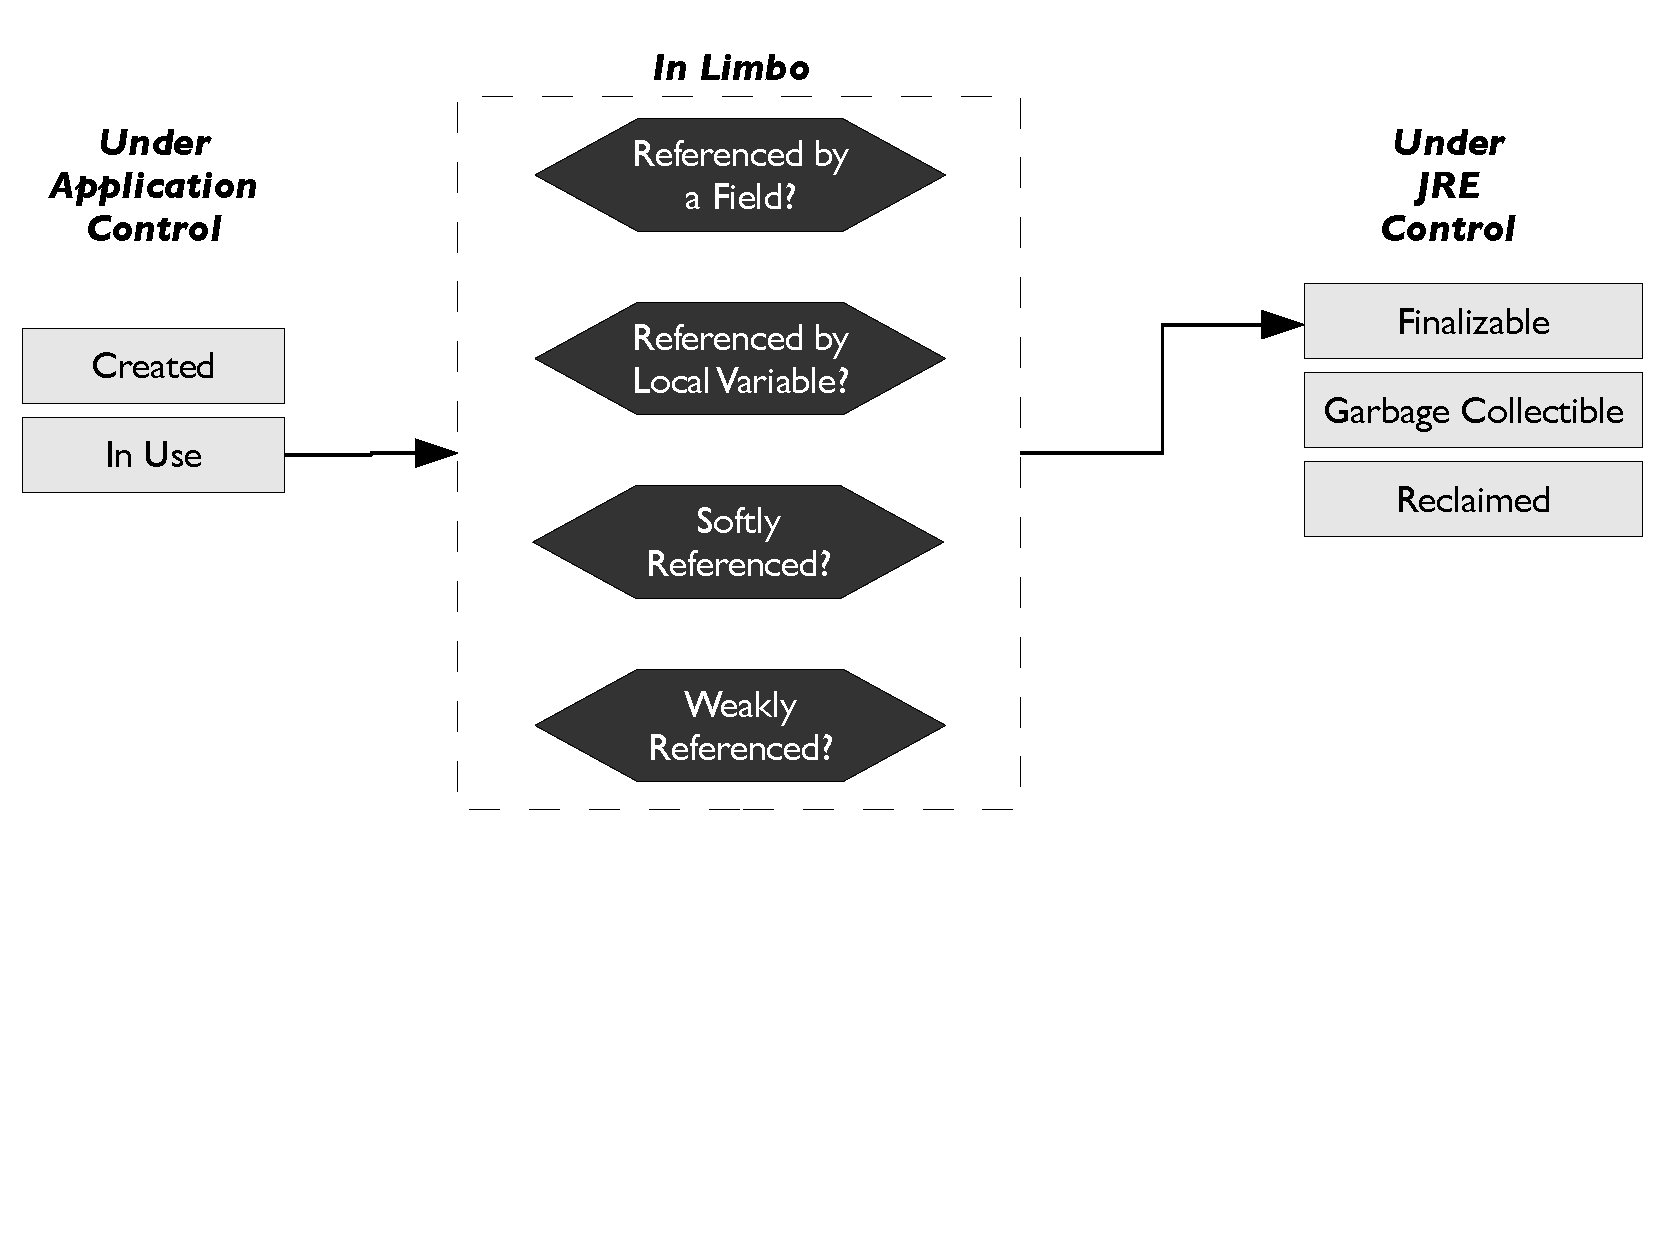
\includegraphics[width=\textwidth]{Figures/lifetime/states}
	\caption{After its last use, an object enters a kind of limbo.}
		\label{fig:limbo-exit}
\end{figure}

\section{Java Lifetime Management Mechanisms} The point at which an object exits
its limbo depends upon how it is referenced by other objects. One can always
assure that an object exits limbo by modifying your code to overwrite all
references to that variable. If an object is no longer referenced at all, then it
will exit limbo immediately.\footnote{Talk about cycles?} For example, a common
way to do this is by assigning references to the value \code{null}. This is
tricky in many cases, because it may not be easy to know where all those
references emanate from. Who is to say that, when one calls the \code{parse}
method of a \class{SimpleDateFormat} object, that it does not squirrel away a
reference to the \class{ParsePosition} passed as a parameter? The API contract
for \code{parse} makes no such claims, one way or the other. This is certainly
calls to mind the worst of the days of explicitly managing memory in a language
like C.


\begin{table}
\centering
	\begin{tabular}{ll} \toprule reachable only from  & \textbf{special condition}
	when object exits limbo \\ \cmidrule(r){1-1} \cmidrule(l){2-2}
			%
			nothing & immediately
        	\\
        	%
        	local variable & next garbage collection after scope exits
        	\\ \addlinespace
        	%
        	instance field of an object & 
        	when that object exits limbo %(could be \emph{never} --- memory leak)
        	\\
        	%
        	static field of an object &
        	when that object's class is unloaded
        	%
        	\\ \addlinespace
        	field of \class{WeakReference} & next garbage
        	collection
        	\\
        	%
        	field of \class{SoftReference} & approximately
        	LRU%$^{**}$
        	%
        	\\
        	entry in thread local storage & when that thread dies
        	%
        	\\ 
        \bottomrule
    \end{tabular}
	\caption{When, or
	even whether, an object exits limbo depends upon how your program references
	it. If these references aren't explicitly overwritten, e.g. by your
	code expliclty assigning the reference to \code{null}, then an object only
	exits limbo under certain restricted circumstances.
%	The point when an object exits limbo depends on 
	%decisions under programmer control: it depends on how the object is
	%referenced.
	%older {\jre}s	use very poor heuristics for handling soft references; see the
	% body for more detail.
	%, it will be reclaimed
	%under certain rules, or may be part of a memory leak
	}
	\label{tab:limbo-exit}
\end{table}

Still, one can't always rely on automatic mechanisms to guide an object out of
limbo in a timely fashion.
\autoref{fig:limbo-exit} and \autoref{tab:limbo-exit}
illustrate how an object may exit limbo. 
A garbage collector only knows that an object is ready to
be collected based on {\em reachability}: how the objects point to eachother.
If, as in the \class{ParsePosition}
or \class{SimpleDateFormat} objects from our example, the object is referenced
only by a local variable of a method, the \jre will not consider reclaming its
storage until the variable's scope exits; e.g. when the loop continues to the
next iteration, or when the method returns, depending on the scope of the
variable that references the object. If the object is referenced only by a
field of another object, then it must wait for that other object to exit limbo
before it can do so. 
An objects pointed to be only by a static field has a good chance of never
being collected. A class only exits limbo when it is unloaded by the \jres
class loading mechanism, which is unlikely to happen if it has static fields
that reference other objects. Therefore, unless that field is overwritten,
objects pointed to by static fields are likely never to exit limbo.

The Java specification provides three other mechanisms that let you guide the
\jre into the right time for an object to exit limbo: weak and soft references,
and thread-local storage.

\subsection{Weak and Soft References}



\subsection{Thread-local References}


\begin{comment}
\begin{figure}
	\centering
	\subfigure[The lifecycle of a typical object and its data.]{
	\label{fig:typical-lifecycle1}
			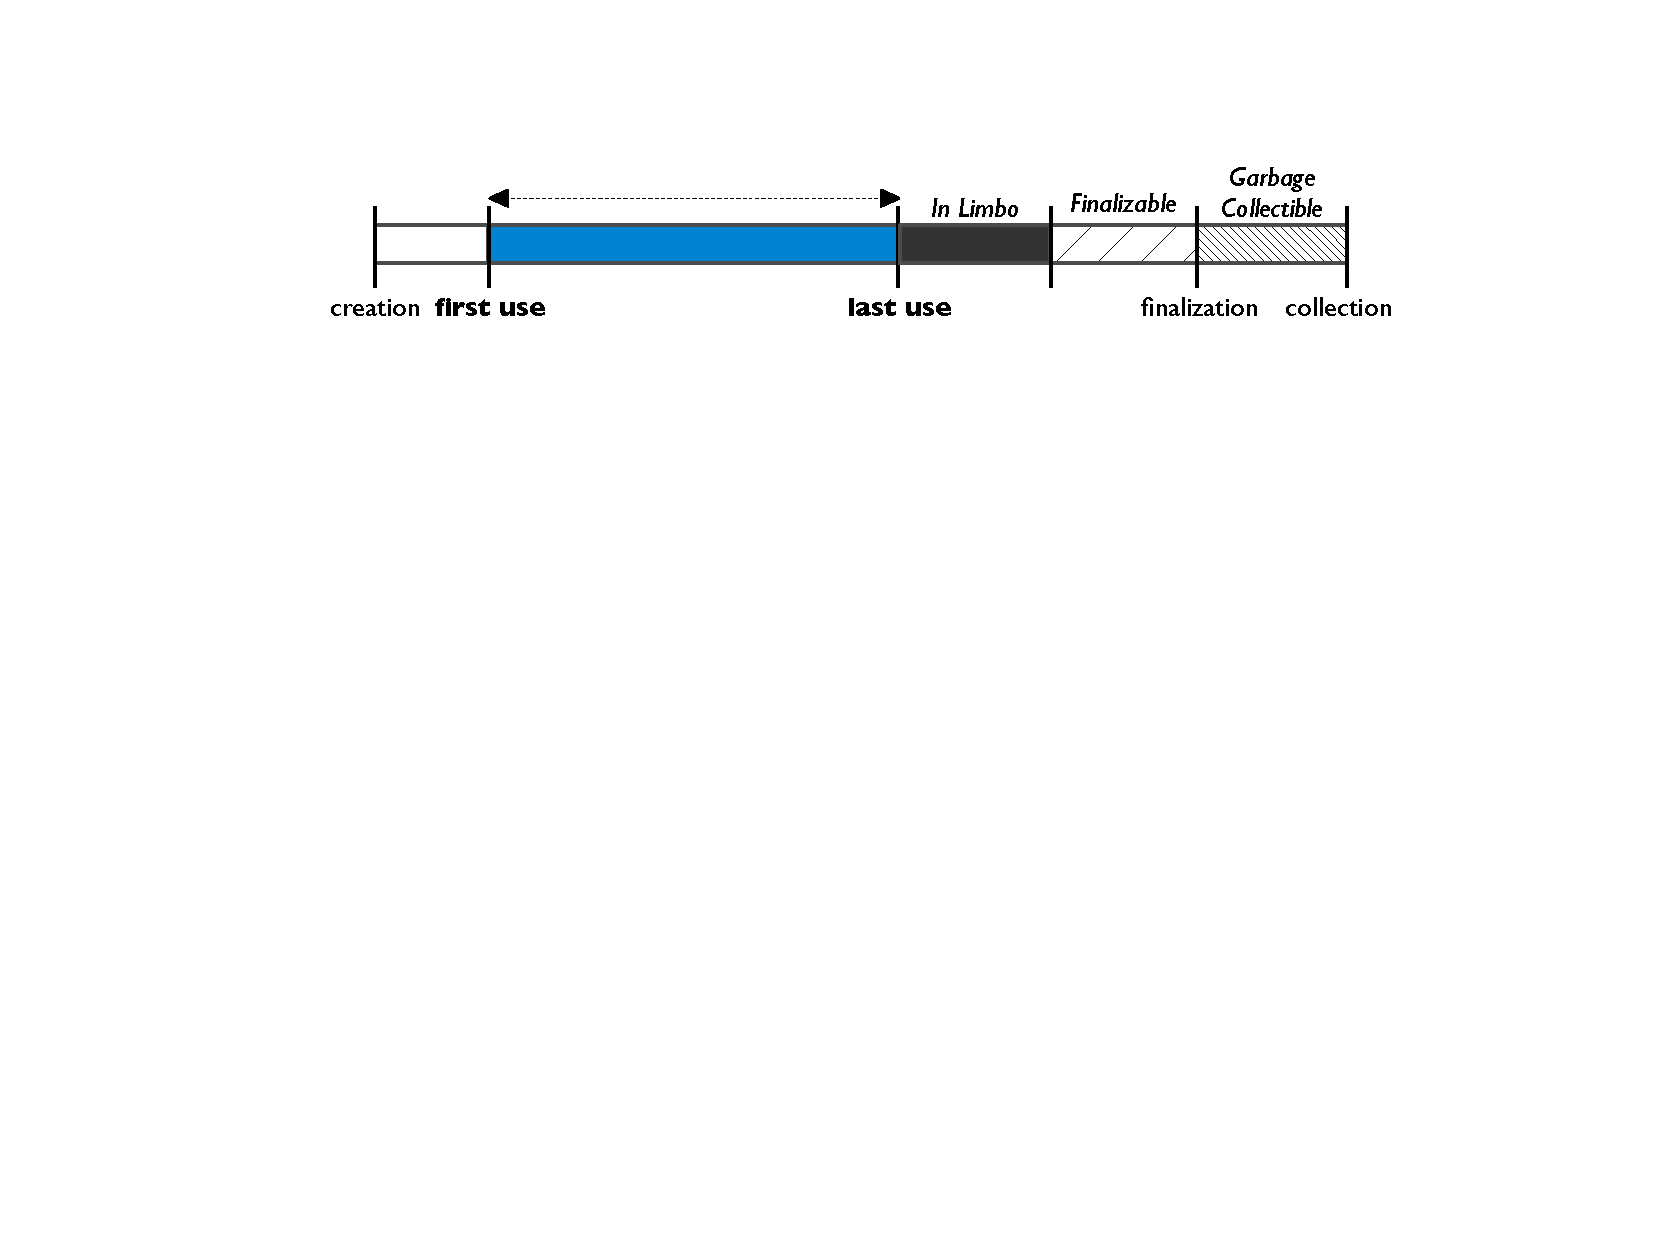
\includegraphics[width=0.95\textwidth]{Figures/lifetime/object-lifecycle}
	}
	\subfigure[A situation where there are long periods between uses of an
	object's data.]{
	\label{fig:typical-lifecycle2}
		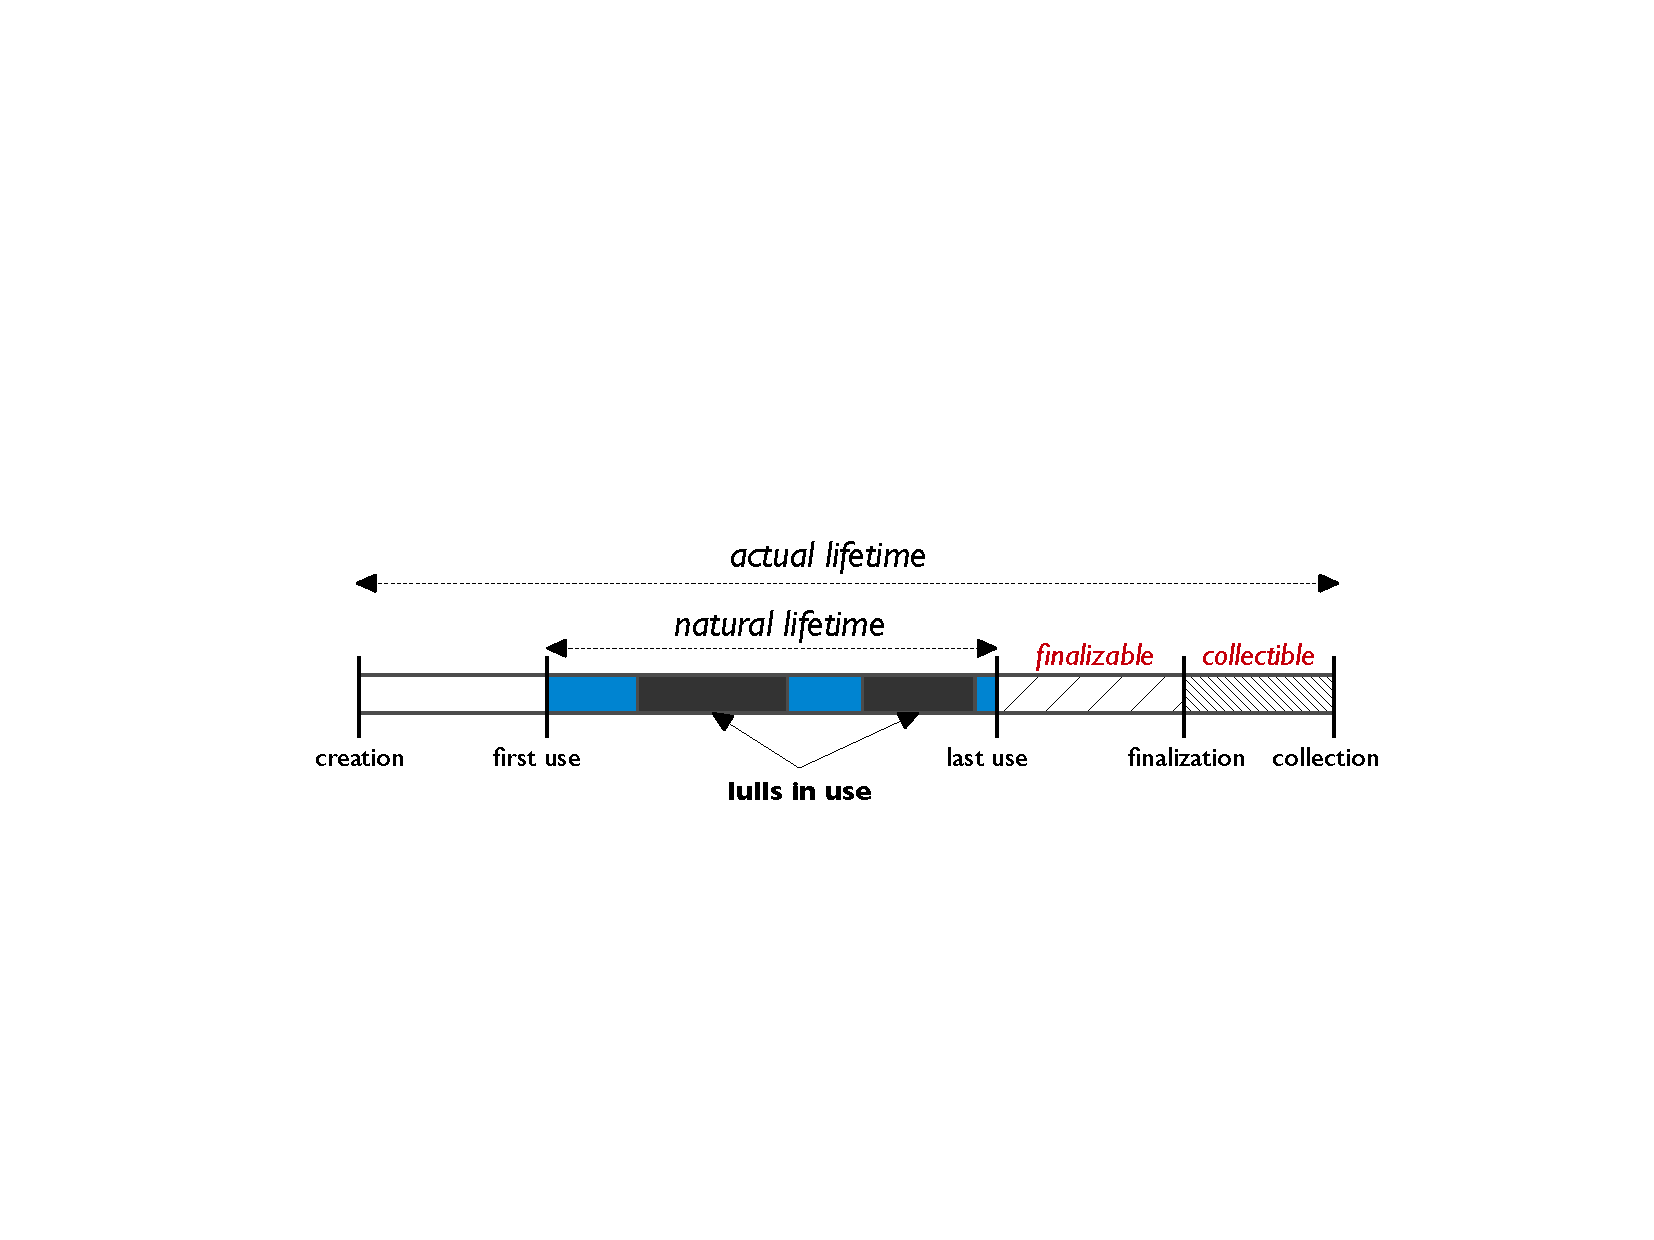
\includegraphics[width=0.95\textwidth]{Figures/lifetme/object-lifecycle-lulls}
	}
	\subfigure[The lifecycle of the data  that is loaded from
	disk three times, and the objects that store it.]{
	\label{fig:typical-lifecycle3}
		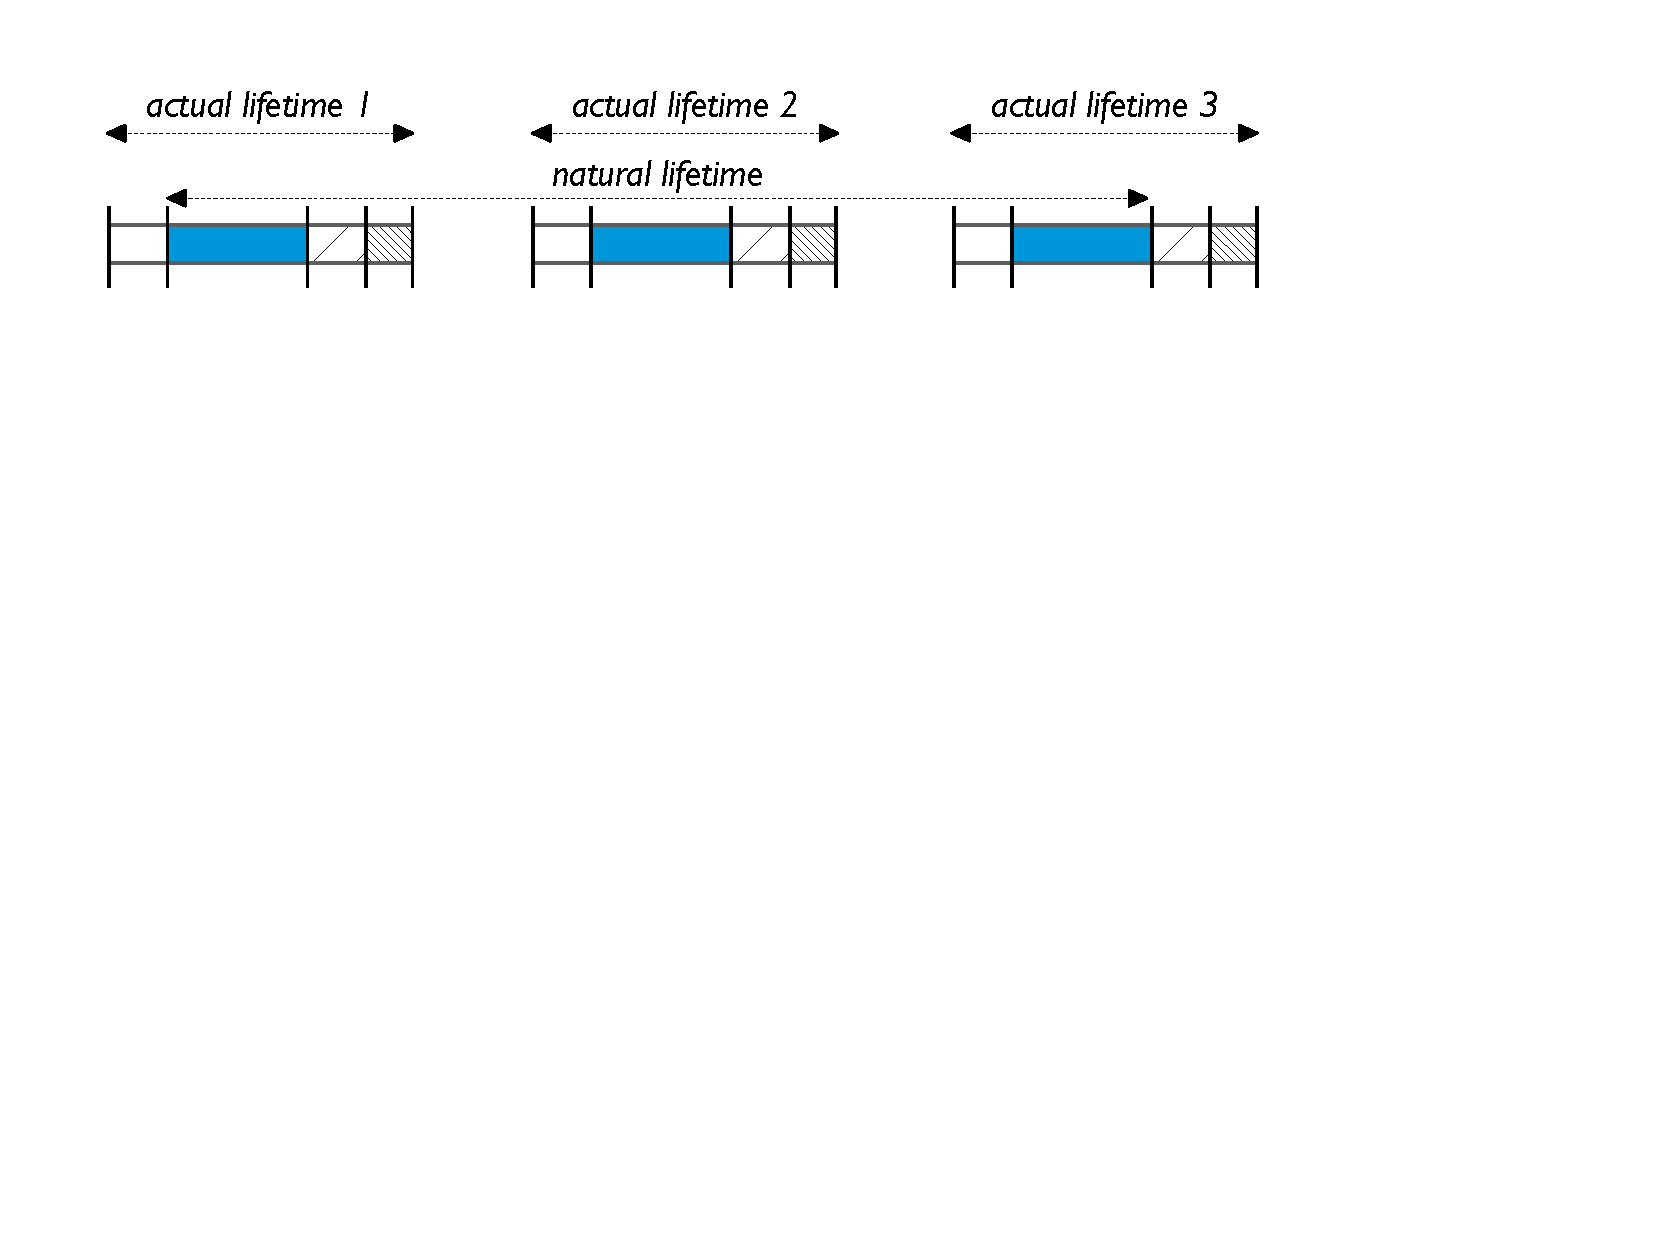
\includegraphics[width=0.9\textwidth]{Figures/object-lifecycle2}
	}
	\caption{Examples of Natural and Actual lifetimes.}
	\label{fig:typical-lifecycle}
\end{figure}
\end{comment}

\section{Common Categories of Natural Lifetime}

\begin{table}
\centering
	\begin{tabular}{lp{0.30\textwidth}p{0.35\textwidth}}
	\toprule  & Lifetime Property & Example \\ \midrule
	\autoref{temporary-lifetime}  & {Temporary} & new
	parser for every date
	\\
	\autoref{forever-lifetime} & {Needed Forever} & product catalog
	\\
	\autoref{correlated-lifetime-1} & {Correlated with Object}
	& object annotations
	\\
	\autoref{correlated-lifetime-2} & {Correlated with Phase} &
	DOM used only parsing
	\\
	\autoref{deferred-deletion} & {Deferred Deletion} &
	session state \\
%period\\ scoped to a phase/request\\
%correlated with an object (annotations)\\
%correlated with need}\\ \hline
%reusable & maybe i'll need it later \\ \hline
	\bottomrule
	\end{tabular}
	\caption{Five important categories of object lifetime.}
	\label{tab:five-lifetimes}
\end{table}

\autoref{tab:five-lifetimes} summarizes five important cases of object lifetime.
% introduced by example in this chapter, and
Many objects are either temporaries or needed for
the entire run of your application. Sometimes you create objects whose lifetime
is correlated with other objects or that should go away when a method invocation
completes. Sometimes you need to manage objects hanging around longer than their
current need, to avoid future recomputations or refetching of data in the case
when it is needed in the near future. 


\begin{table}
\centering
	\begin{tabular}{ll} \toprule
    	& Things Java Doesn't Do Automatically \\ \midrule
    	\autoref{avoiding-lifetime-bugs} & {Avoiding Memory Leaks} \\
    	\autoref{balance-time-and-space} & {Balancing Time and Space} \\
    	\autoref{outisde-java-box} & {Supporting Massive Data Sets}  	\\
        \bottomrule
    \end{tabular}
	\caption{Elements of programming for which Java's built-in mechanisms don't
	provide great support.}
	\label{tab:things-java-does-not-do}
\end{table}


\section{Temporary Objects}
\label{temporary-lifetime}

If your application is like most Java applications, it creates a large number of
temporary objects. They hold data that will only be used for a very short
interval of time. For example, you populate a \class{StringBuffer}, turn it into
a \class{String}, and print the string to a log file. The point at which all of
these objects, the strings and character arrays, are no longer used is only
shortly after they are constructed. These objects serve as transient homes for
your data, as it makes its way through the frameworks and libraries you depend
on. Temporaries are often necessary to bridge separately developed code and
enable code reuse: as long as you can convert your data layout into a form that
an API requires, then you can reuse the functionality it provides.

In many cases, you need do nothing special to manage the temporary objects your
application creates. After all, generational garbage collectors these days do a
very good job digesting a large volume of temporary objects. In a generational
garbage collector, the \jre places temporary objects in a separate heap, and
thus it need only process the newly created objects during its routine scan.
Unfortunately, in Java it is pretty easy to create a high volume of temporary
objects. Say your application 
fills it the temporary heap ever second. In this case, based on the common
speeds of garbage collectors, your application could easily spend over 20\% of its time
collecting garbage.
Is it difficult to fill up the temporary heap once per second? Typical
temporary heap sizes run around 128 megabytes. Say your application is a serves
a peak of 1000 requests per second, and creates objects of around 50 bytes each.
Then it need only create around 2500 temporaries per request. 


%A great many of these
%temporary structures serve the role of a kind of lubricant, making it easy for
%you to write code that ties together the separately written parts of your code
%base and reuses standard libraries as much as possible. Often, these are
%objects that are not a fundamental necessity of what you're trying to
%accomplish. If
%you had the freedom to code highly specialized implementations of the important
%cases, from scratch, many of these temporary structures would be unnecessary.

\begin{example}[How Easy it is to Create Lots of Temporary Objects]
A common example of temporaries is parsing
and manipulating data coming from the outside world. 
% to the wire?
Consider the code in \autoref{TempExampleCode}. This code starts in
the \code{main} method by splitting the input string into two substrings. So
far, the code has created four objects (one \class{String} and one character
array per substring). 
Creating these substrings makes it easy to use the \code{doWork} method, which
takes two Strings as input. However, observe
that these four objects are not a necessary part of the computation. Indeed,
these substrings are eventually used only as input to the
\class{SimpleDateFormat} \code{parse} method, which has been nicely designed to
allow you to avoid this very problem. By passing a \class{ParsePosition}, one
can parse substrings of a string without having to create temporary strings (at
the expense of creating temporary \class{ParsePosition} objects!).



\begin{lstlisting}[float,caption=Code that constructs 8 temporary objects to handle two dates.,label=TempExampleCode]
void main(String xy) {
	doWork(xy.substring(0,10), xy.substring(10));
}	
void doWork(String x, String y) {
	doRemoveProcedureCall(parse(x));
	doRemoveProcedureCall(parse(y));
}
	
Date parse(String string) {
	return new SimpleDataFormat().parse(string, new ParsePosition(0));
}

void doRemoteProcedureCall(Date date) {
	long timestamp = date.getTime();
	...
}
\end{lstlisting}

\end{example}

% correlated with need: as soon as last user goes away, remove his stuff 
% share common expressions to save space, but using strong references -> memory
% leak; plugins in eclipse go away when all views
% sharing pool 

% weak ref keys -> annotation
% weak ref values -> sharing pool

% soft ref values -> caching

% annotation by map lookup


\section{Objects Needed Forever}
\label{forever-lifetime}

Created and used for the remaining duration of a run.


\section{Objects with Correlated Lifetimes}

Many objects are created and then only needed for some interval of time. For
example, say your application is a transaction processing system implemented as
a Java Enterprise Edition web application. In this case, most objects
created within the scope of a servlet request will not, and for correctness
reasons {\em must not}, survive the request; they are not used by the 
application after the request has completed, and will, in the absence of bugs,
be collected as soon as is convenient for the runtime. In this example, the
lifetime of objects during a request are {\em correlated} with a method
invocation: when the servlet \class{doGet} or \class{doPut} (etc.) invocations
return, those correlated objects had better be garbage collectible.

The same is true for a great many objects created by the application, not just
at the large granularity of a servlets. For example,

In many cases, the built-in mechanisms 

\subsection{Correlated with Another Object}
\label{correlated-lifetime-1}

\subsection{Correlated with Need}
\label{correlated-lifetime-2}

\section{Objects with Deferred-Deletion}
\label{deferred-deletion}

A cache is a performance optimization that holds on to a data structure after the
current operation is finished with it, in the hope that other operations in the
near future will reuse it. The expense of re-fetching data from external data
sources and recomputing the in-memory structure can often be amortized, at the
expense of stretching the lifetime of these data structures. By increasing the
actual lifetime on an object you will very likely increase peak memory
consumption.




%if scopes don't coincide with lifetime





%% OLD STUFF NMM 20090820
%\section{Request Scoping}
%\section{Correlated Lifetime}
%\paragraph{Weak and Soft references in Java}
%\section{Memory Leaks and Drag}
%\section{Examples}
%\subsection{Transient Near-Copies}
%\subsubsection{String Canonicalization}
%\subsection{Temporary Collections}
%\subsection{Facilitators}
